\documentclass[preprint,12pt,authoryear,a4paper]{elsarticle}
% Shared preamble of the manuscript and the supplementary material (elsarticle, XeLaTeX via tectonic).
\usepackage{fontspec}
\setmainfont{texgyretermes}[Extension=.otf,UprightFont=*-regular,BoldFont=*-bold,ItalicFont=*-italic,BoldItalicFont=*-bolditalic]
\setsansfont{texgyreheros}[Extension=.otf,UprightFont=*-regular,BoldFont=*-bold,ItalicFont=*-italic,BoldItalicFont=*-bolditalic]
\usepackage{amsmath}
\usepackage{unicode-math}
\setmathfont{texgyretermes-math.otf}
% a text block close to the journal's printed figure width (19 cm): figures print near their drawn size
\usepackage[a4paper,left=2.4cm,right=2.4cm,top=2.4cm,bottom=2.6cm,footskip=1cm]{geometry}
\usepackage{graphicx}
\graphicspath{{figures/}}
\usepackage{booktabs}
\usepackage{array}
\usepackage{tabularx}
\usepackage{longtable}
\usepackage{pdflscape}
\usepackage{rotating}
\usepackage{xcolor}
\usepackage{setspace}
\usepackage{lineno}
\usepackage[labelsep=period,labelfont=bf,font=small,justification=justified,singlelinecheck=false]{caption}
\usepackage{placeins}
\usepackage[hidelinks]{hyperref}
% citation links inside floats are misplaced by the PDF driver (xdvipdfmx): floats carry no links
\usepackage{etoolbox}
\AtBeginEnvironment{figure}{\NoHyper}
\AtBeginEnvironment{table}{\NoHyper}
\AtBeginEnvironment{sidewaystable}{\NoHyper}
% references as the journal prints them: DOIs as https://doi.org/..., no 'URL:' prefix, URLs in the text font
\urlstyle{same}
\providecommand{\DOIprefix}{}\renewcommand{\DOIprefix}{}
\providecommand{\URLprefix}{}\renewcommand{\URLprefix}{}
\providecommand{\doi}[1]{}\renewcommand{\doi}[1]{\url{https://doi.org/#1}}
\providecommand{\hy}{-}  % a hyphen that the bibliography style does not turn into a dash
\renewcommand{\figurename}{Fig.}
\newcolumntype{L}[1]{>{\raggedright\arraybackslash}p{#1}}
\newcolumntype{Y}{>{\raggedright\arraybackslash}X}
\newcolumntype{R}[1]{>{\raggedleft\arraybackslash}p{#1}}
\setlength{\tabcolsep}{4pt}
\setlength{\emergencystretch}{3em}  % fewer overfull lines in the justified text
% notes set below a table body
\newcommand{\tablenotes}[1]{\par\smallskip{\footnotesize\raggedright #1\par}}
\journal{NeuroImage}

\begin{document}

\begin{frontmatter}

\title{Sensor noise, array design and helmet fit in on-scalp and cryogenic magnetoencephalography: a simulation study from adults to children}

\author[a]{Laiba Khan}
\author[b]{Mainak Jas\corref{cor1}}
\ead{mjas@mgh.harvard.edu}
\cortext[cor1]{Corresponding author.}
\address[a]{Lexington High School, 251 Waltham Street, Lexington, MA 02421, USA}
\address[b]{Athinoula A. Martinos Center for Biomedical Imaging, Massachusetts General Hospital and Harvard Medical School, 149 Thirteenth Street, Charlestown, MA 02129, USA}

%% HIGHLIGHTS-BEGIN
\begin{highlights}
\item Array design, OPM noise and the SNR measure decide whether OPMs outperform SQUIDs
\item The modeled dense-array advantage is as large as the model's error for SQUID noise
\item Break-even OPM white noise is 31.5 fT/√Hz for a dense array, 16.7 at the SQUID sites
\item Fitting the SQUID helmet removes most of the extra OPM advantage in smaller heads
\item With an idealized detector, dense OPMs detect weaker simulated superficial spikes
\end{highlights}
%% HIGHLIGHTS-END

%% ABSTRACT-BEGIN
\begin{abstract}
Optically pumped magnetometers (OPMs) worn on the scalp sit closer to the brain than the sensors of cryogenic magnetoencephalography (MEG), but whether they detect cortical sources better depends on noise, which spherical-head analyses reduce to an assumed ratio. Here, we compared the 306-channel Neuromag system with two single-axis OPM arrays (208 dense sites; Neuromag's 98 sensor sites) by matched-filter detectability with explicit sensor, brain and room noise, in an adult and in smaller heads in the adult helmet or a helmet fitted to the adult's gap. In the adult, the dense array's detectability was 1.14 times Neuromag's (95 % parcel-bootstrap interval [1.12, 1.17]) up to a break-even OPM noise of 31.5~fT/√Hz; the site-matched array broke even at 16.7~fT/√Hz. With Neuromag's measured noise covariance, the dense ratio was 1.03 [0.99, 1.08], so measured OPM noise must decide the adult comparison. In two scaled copies of the adult and three infant templates, the fixed adult helmet added +0.44 to +1.07~dB to the OPM advantage, and fitting the helmet removed +0.40 to +1.10~dB of this excess, a contrast that depends on the SQUID helmet alone. Under the modeled noise and with an idealized detector, the dense array detected simulated superficial interictal spikes at 21–32\,\% lower strength than Neuromag in every head, without a localization difference. Three school-aged children with unverified near-scalp anatomy gave provisional results. In this model, array design, OPM noise and the fit of the SQUID helmet, not proximity alone, determine the on-scalp advantage.
\end{abstract}
%% ABSTRACT-END

\begin{keyword}
Magnetoencephalography (MEG) \sep Optically pumped magnetometer (OPM) \sep Superconducting quantum interference device (SQUID) \sep Pediatric neuroimaging \sep Helmet fit \sep Noise covariance \sep Interictal spikes
\end{keyword}

\end{frontmatter}

\linenumbers

%% =====================================================================
\section{Introduction}\label{sec:intro}

Optically pumped magnetometers (OPMs) measure the brain's magnetic field at room temperature and can be worn on the scalp, whereas the superconducting quantum interference devices (SQUIDs) of conventional magnetoencephalography (MEG) sit in a rigid cryogenic helmet \citep{boto2017,iivanainen2017}. The helmet is built for adults, so a child's head sits in it with a wide and uneven gap, whereas an on-scalp array can fit any head \citep{feysdetiege2024,hill2019}. Clinical OPM studies of epilepsy report larger interictal discharges than cryogenic MEG \citep{feys2022}. Their signal-to-noise ratios (SNRs) were higher in some comparisons (\citealp{feys2022,feys2025}; \citealp[abstract only]{ren2025}) and equal or slightly lower in others \citep{hillebrand2023,schwartz2025}, and their weakest results concern temporal and mesial temporal sources \citep{feys2024,feys2025,shen2026}.

A larger field does not by itself give a higher SNR, because an OPM is a noisier sensor than a SQUID magnetometer. A spherical-head analysis made this explicit with a point magnetometer on the scalp (OPM) and one 18~mm above it (SQUID) \citep{jas2026}. For intermediate ratios of OPM to SQUID noise, the OPM's single-channel SNR was higher only for sources shallower than an equal-SNR depth, about 28~mm in an adult head when the OPM's noise was 3 times the SQUID's. With a SQUID shell that follows the head at a constant standoff, this depth covers a larger fraction of a small brain, which predicts a larger OPM benefit in children.

A realistic comparison needs explicit noise seen through each array's own lead fields, finite arrays on a real scalp, and a real helmet around a smaller head. With sensor noise only, an array of helium-4 OPMs gained on SQUID magnetometers as the head shrank, both in a standard adult placement and in a helmet fitted at a constant gap \citep{zahran2022}. With brain noise in one adult, simulated spikes were visible on the scalp from smaller cortical patches with on-scalp than with conventional MEG \citep{westin2023}. With brain noise but no sensor noise, OPMs placed at the SQUID sites of epilepsy patients raised a channel-averaged SNR in no region, although the OPM--SQUID difference followed the ratio of sensor distances, which tracked head circumference \citep{matsubara2026}.

These studies leave three gaps. None compared head size and helmet fit with brain noise included, and none checked its noise model against a measured covariance. The one helmet fitted at a constant gap was fitted at the adult's closest distance \citep{zahran2022}, not at the adult's median gap. It is therefore unknown whether the larger OPM advantage expected in children reflects the small head itself or the poor fit of the adult helmet. It is also unknown how far a modeled comparison can be trusted while the OPM's noise has not been measured in the same conditions.

Here, we compared the 306-channel Neuromag system with a dense and a site-matched OPM array in a realistic adult head and in smaller heads, using matched-filter detectability with explicit sensor, brain and room noise. We asked four questions. First, what decides the comparison in the adult, and how far can the noise model be trusted when it is checked against Neuromag's measured noise? Second, which brain regions favor the OPM, and where does an array at Neuromag's sites fall behind (exploratory)? Third, is the larger relative advantage in smaller heads a matter of head size or of the fixed adult helmet? We tested this with a helmet fitted to each head at the adult's gap. Fourth, does the detectability difference carry over to the detection of simulated interictal spikes by an idealized detector, and to their localization (exploratory)?

%% =====================================================================
\section{Materials and methods}\label{sec:methods}

\subsection{Study design and estimands}\label{sec:design}

We compared arrays by known-topography detectability, the output SNR of the matched filter for a source of known field pattern in noise of known covariance:
\begin{equation}
d = \sqrt{\symbf{s}^{\top}\symbf{C}^{-1}\symbf{s}},
\label{eq:d}
\end{equation}
where $\symbf{s}$ is the noise-free field of a 10-nAm cortical dipole at the array's channels and $\symbf{C}$ is the array's noise covariance (Section~\ref{sec:noise}), taken as known (the oracle covariance). For each target, two arrays were compared by the ratio $d_{\mathrm{OPM}}/d_{\mathrm{Neuromag}}$ or, in decibels, by
\begin{equation}
D = 20\log_{10}\frac{d_{\mathrm{OPM}}}{d_{\mathrm{Neuromag}}},
\label{eq:D}
\end{equation}
which is positive when the OPM array detects the source better.

For the adult, we summarize the target-wise ratios by their unweighted median over all 7,661 targets, including the 558 on the medial wall, which is not cortex; this is the adult analysis's declared convention, and without them the dense array's ratio is 1.15. The smaller heads differ in cortical area, so for each of them we summarize $D$ by its area-weighted median over cortical targets, medial wall excluded. A smaller head's change from the adult, $\Delta$, is the area-weighted median of paired target-level differences in $D$, with the adult placed by the same helmet rule; it is not the difference of the two heads' medians. Targets are paired per vertex for the scaled adults, which share the adult's vertices, and per atlas parcel for the other heads. Intervals are 95\,\% percentile bootstrap intervals over atlas parcels (Section~\ref{sec:stats}).

\subsection{Head models}\label{sec:heads}

The adult head was the MNE sample subject \citep{gramfort2013}, with FreeSurfer surfaces and atlas labels \citep{desikan2006,fischl2012}. Targets were the vertices of an MNE-Python oct-6 source space (a recursively subdivided octahedron) on the white-matter surface lying at least 4~mm inside the inner skull, each a 10-nAm dipole normal to the cortex. A target's depth was its distance to the nearest point of the MRI scalp. A three-layer boundary-element model (BEM; \citealp{hamalainen1989}) with conductivities of 0.3, 0.006, 0.3~S/m had its outer surface on the MRI scalp.

The eight smaller heads fell into three classes (Table~\ref{tab:anatomies}), which carry different weight. The two scaled adults are copies of the adult scaled to school-age size and to the head circumference of the 24-month template; they keep the adult's anatomy exactly and carry the comparison of head size and helmet fit. The three infant templates, at 24, 18 and 12 months, are averages of many MRIs \citep{oreilly2021,richards2016}; they add infant head shapes, with the qualifications given below. The three typically developing school-aged children, A, B and C (7.8–8.7 years), came from OpenNeuro dataset ds005234 \citep{fadeev2024,fadeev2025} and are reported as provisional examples. The anatomies are therefore not independent replications, and all of them share the noise calibration, the adult's conductivities and the processing.

The children's anatomy needed three further steps (Section~S4). First, the dataset's BEM surfaces placed the inner skull a median of 0.8–2.5~mm below the scalp over the upper head, implausibly close. We moved it inward toward 8~mm below the scalp wherever it lay shallower, keeping every inner-skull vertex at least 2~mm from the white-surface vertices, so that over the upper head it lay a median of 5.7–7.8~mm below the scalp (adult, 9.7~mm). Between vertices, the inner skull came within 0.9–1.3~mm of the white surface, and in child B the outer skull came within 0.17~mm of the scalp. A single-compartment BEM, which needs no skull, changed the difference between each smaller head's median $D$ and the adult's by −0.06 to +0.01~dB.

Second, no fiducials come with these data. We transferred them from the adult by a similarity transform fitted between the adult's and the child's white surfaces (trimmed iterative closest points) and moved each to the nearest scalp vertex. Applied to the infant templates, this method reproduced their own fiducials with errors of 1.6–14.4~mm and their head frames with rotations of 3.2–5.9°. Third, because the children's white surfaces came within 3.7–5.7~mm of the scalp, we checked the surfaces against their T1-weighted MRIs (Fig.~S6). The FreeSurfer scalp lay about as far inside the T1 head boundary in the children (median 1.3–1.5~mm) as in the adult (1.3~mm), and the white surfaces were registered to the T1 images. Relative to these images, the shallow cortex is therefore not a scalp-placement or registration error.

The count of shallow targets depends on the scalp definition: measured to the MRI head boundary, child B has 47 rather than 247 targets less than 10~mm deep. The source rule left out 3.3–10.0\,\% of the children's cortex (adult, 7.2\,\%), including 94–100\,\% of their cortex within 8~mm of the scalp. The infant templates' scalps lay 1.3–1.6~mm outside their own MRI head boundaries, whereas the adult's lies inside. The check also classed the 18-month template as misregistered: its white surface fitted its T1 image best after a 2.3-mm shift (0.5~mm in the other two templates).

\begin{table}[tbp]
\caption{Head models.}\label{tab:anatomies}
\centering\footnotesize
\begin{tabular}{L{3.0cm}L{2.4cm}R{2.1cm}R{1.6cm}R{1.4cm}R{2.4cm}}
\toprule
Head & Class & Head circumference (cm) & Cortex (cm$^{2}$) & Targets & OPM sites, dense / site-matched \\
\midrule
Adult & MNE sample subject & 58.6 & 1,878 & 7,103$^{\mathrm{a}}$ & 208 / 98 \\
School-age size & scaled adult & 52.5 & 1,470 & 6,949 & 174 / 89 \\
2-year size & scaled adult & 49.5 & 1,290 & 6,855 & 155 / 90 \\
24-month template & infant template & 49.5 & 1,062 & 7,559 & 151 / 83 \\
18-month template$^{\mathrm{b}}$ & infant template & 49.1 & 975 & 7,363 & 157 / 80 \\
12-month template & infant template & 46.9 & 895 & 7,592 & 144 / 82 \\
Child A (7.8~years) & school-aged child$^{\mathrm{c}}$ & 52.0 & 1,852 & 7,138 & 155 / 90 \\
Child B (8.3~years) & school-aged child$^{\mathrm{c}}$ & 48.6 & 1,666 & 6,866 & 153 / 85 \\
Child C (8.7~years) & school-aged child$^{\mathrm{c}}$ & 53.5 & 1,869 & 7,392 & 167 / 91 \\
\bottomrule
\end{tabular}
\tablenotes{Head circumference is that of the MRI scalp; cortex is the usable cortical area; targets exclude the medial wall. The median magnetometer-to-scalp gaps of each head in each helmet, with the fitted helmets' scale factors, are listed in Table~S5. Infant templates: \citet{oreilly2021}, from the Neurodevelopmental MRI Database \citep{richards2016}. Children A--C: OpenNeuro ds005234 \citep{fadeev2024,fadeev2025}. $^{\mathrm{a}}$The adult's whole-cortex medians use all 7,661 targets, the medial wall included (Section~\ref{sec:design}). $^{\mathrm{b}}$Classed misregistered by the MRI check (Section~\ref{sec:heads}). $^{\mathrm{c}}$Provisional examples: near-scalp anatomy not verifiable (Section~\ref{sec:heads}).}
\end{table}

\subsection{Sensor arrays and helmets}\label{sec:arrays}

The Neuromag system (306 channels; ``Neuromag'' below) combined the sample recording's VectorView sensor geometry with the T3 coil definitions of MNE-Python (types 3014 and 3024). Its white noise was the typical value of the TRIUX datasheet, 3.5~fT/√Hz for the magnetometers and 3.6~fT/(cm~√Hz) for the gradiometers, with an 18-mm Dewar spacing between coils and helmet surface \citep{elekta_triux}. No signal-space separation was applied.

Each OPM was a single-axis sensor whose sensing center lay nominally 7~mm above the MRI scalp \citep{alem2023,osborne2018}, with a few sites moved outward for clearance. Its field was averaged over a 10-mm cubic volume, a modeling choice that changes the peak field by at most 1.9\,\%. Its sensitive axis was the head-surface normal averaged within 15~mm of the site; with nearly radial axes, the dense array's ratio with the room field projected out (Section~\ref{sec:noise}) would be 1.07 instead of 1.12 (Section~S3).

OPMs covered the scalp above the plane through the preauricular points and a point 30~mm above the nasion, keeping at least 20~mm from either preauricular point. The dense OPM array filled this region at a minimum spacing of 17~mm (208 sites on the adult, more sites than any clinical OPM array). The site-matched OPM array placed one OPM at each Neuromag site whose projection onto the scalp fell inside it (98 of 102 sites; Fig.~\ref{fig:arrays}). On every smaller head, the dense array was rebuilt by the same rules (144–174 sites), and the site-matched array took that head's Neuromag sites at top contact (80–91 sites; Table~\ref{tab:anatomies}).

Clinical systems reach about 100--128 channels with dual- or triaxial sensors at fewer sites \citep{feys2025,shen2026}. We did not model such arrays: the site-matched array, with fewer and single-axis sensors, is a pessimistic proxy for them and the dense array an optimistic one. A triaxial array at the site-matched sites (294 channels) served as a control for the gain from extra axes. The OPM white noise was 15~fT/√Hz in the primary analysis, flat over 1–40~Hz, and was varied over 7, 10, 15, 20 and 30~fT/√Hz.

The fixed adult helmet kept the adult's sensors and noise for every head (Fig.~\ref{fig:helmets}). In its primary placement, top contact, the head was taken from the pose that puts its head frame where the adult's was recorded and raised until the nearest magnetometer coil was 20~mm from the scalp, a best-fit assumption that favors Neuromag \citep{gaetz2008,tesan2010}. A family of 12 source-blind placements, chosen from the geometry alone (contacts, shifts and rotations; Section~S5), gave a placement band.

To separate head size from helmet fit, we also placed each head in a helmet fitted at the adult's gap. The head was moved sideways onto the helmet's midline (laterally centered), and the helmet was scaled about the head origin until the median magnetometer-to-scalp gap equaled the adult's in the same pose, 29.6~mm. For comparison, the adult's gap is 29.8~mm at its measured head position and 28.4~mm at top contact. No coil could come within the 18-mm Dewar spacing of the scalp; in child C, this limit bound first, at 32.8~mm. The fitted helmet keeps the adult's sensors and does not model a pediatric SQUID system.

The primary helmet-fit quantity is the interaction: a smaller head's within-head contrast, the area-weighted median of the target-wise difference in $D$ between the fixed and the fitted helmet, minus the adult's. Both contrasts compare two Neuromag helmets around the same OPM array, so the OPM terms cancel target by target, and the interaction does not depend on the assumed OPM noise. Three secondary controls were a variant fitted at the adult's top-contact gap (28.4~mm), a helmet scaled with the head, which scales the gap too, and an equal OPM site count (Section~S5). For the last, the adult's dense array was subsampled to each smaller head's number of sites.

\begin{figure}[tbp]
\centering
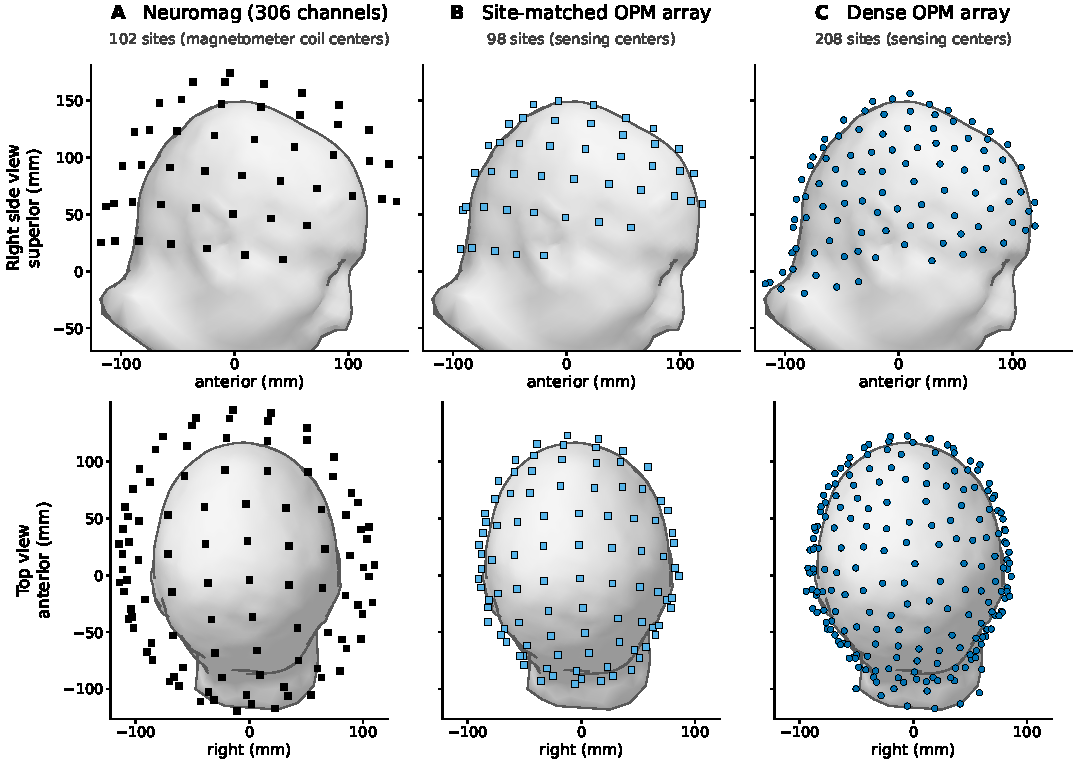
\includegraphics[width=\textwidth]{Figure_1.pdf}
\caption{Sensor arrays on the adult head (MNE sample subject), viewed from the right (sensors on the right half of the head) and from above. (A) Neuromag (306 channels): 102 sites, each holding one magnetometer and two planar gradiometers, at the adult's measured head position (median 29.8~mm from the scalp). (B) Site-matched OPM array: the 98 Neuromag sites inside the OPM coverage region, projected onto the scalp. (C) Dense OPM array: 208 sites at least 17~mm apart. OPM sensing centers lie nominally 7~mm from the scalp and measure the field normal to the head surface.}
\label{fig:arrays}
\end{figure}

\begin{figure}[tbp]
\centering
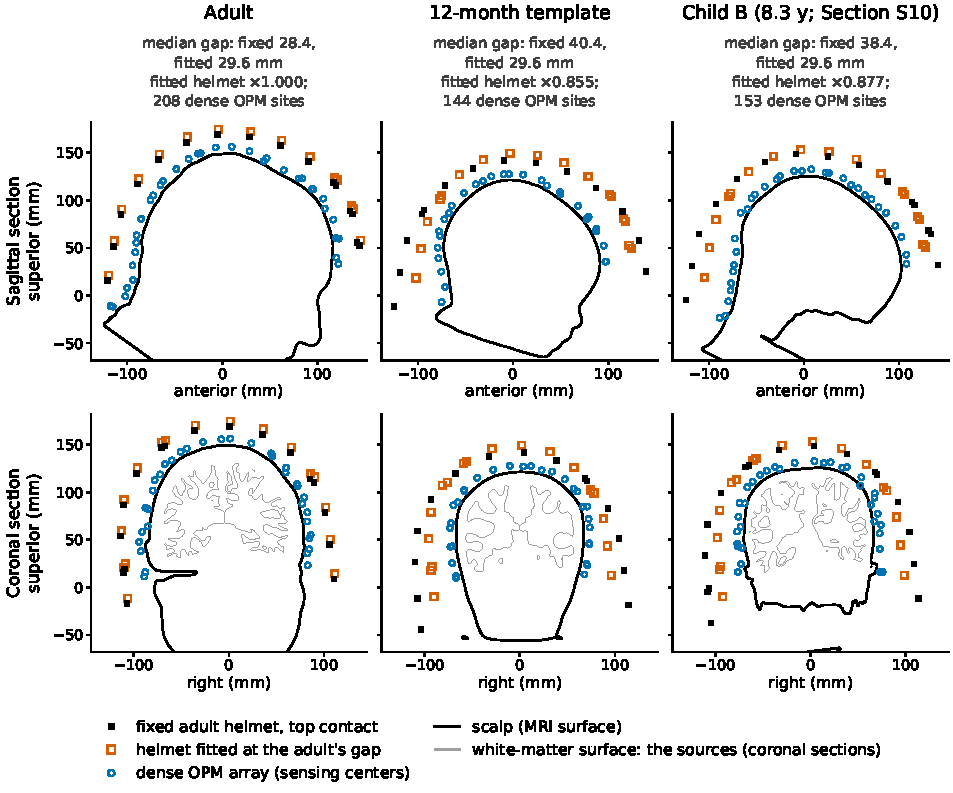
\includegraphics[width=\textwidth]{Figure_2.pdf}
\caption{The fixed and the fitted helmet. Sagittal and coronal sections through the head origin of the adult, the 12-month template and child B, at one scale: scalp (black) and, in the coronal sections, white-matter surface (gray); filled black squares, the Neuromag magnetometers of the fixed adult helmet at top contact; open vermillion squares, the helmet fitted at the adult's gap (scale factor above each column); open blue circles, the dense OPM sites; only sensors within 20~mm of the section are drawn. Median magnetometer-to-scalp gap: 28.4, 40.4 and 38.4~mm in the fixed helmet; 29.6~mm in the fitted helmet. The children's modeled skull is shown against their MRIs in Fig.~S6A. Infant template: \citet{oreilly2021}, from the Neurodevelopmental MRI Database \citep{richards2016}; child B: OpenNeuro ds005234 \citep{fadeev2024,fadeev2025}.}
\label{fig:helmets}
\end{figure}

\subsection{Noise model, validation and sensitivity analyses}\label{sec:noise}

Every array saw identical noise sources in one band of 1–40~Hz. Each array's oracle covariance was computed in closed form as
\begin{equation}
\symbf{C} = \symbf{\Sigma}_{\mathrm{n}} + \sigma^{2}\,\symbf{L}\symbf{A}\symbf{L}^{\top} + \symbf{E}\symbf{\Sigma}_{\mathrm{e}}\symbf{E}^{\top},
\label{eq:C}
\end{equation}
where $\symbf{\Sigma}_{\mathrm{n}}$ is the diagonal covariance of white sensor noise; $\symbf{L}$ holds the lead fields of 1,755 independent cortex-normal background dipoles on a 7-mm grid, and $\symbf{A}$ is the diagonal matrix of their Voronoi-cell areas; and $\symbf{E}$ and $\symbf{\Sigma}_{\mathrm{e}}$ are the array's responses to eight external-field terms (three uniform and five linear-gradient components, the room field) and their coefficient covariance. The background is a cortically constrained form of the random-dipole model of spontaneous activity \citep{demunck1992}: each background dipole's moment variance is $\sigma^{2}$ times its area ($\sigma^{2}$ = 0.0354~nAm$^{2}$ per mm$^{2}$). Like the targets, the background omitted the cortex within 4~mm of the inner skull.

Two quantities were fitted to the sample dataset: $\symbf{\Sigma}_{\mathrm{e}}$, to its empty-room recording, and the scalar $\sigma^{2}$, so that the median good gradiometer's modeled brain noise matched the measured one (a root-mean-square value of 37.1~fT/cm). Apart from the declared sensor noise of both systems, everything else is a prediction. We analyzed four noise conditions: sensor noise only; sensor plus brain noise, the primary condition; sensor, brain and room noise; and the last with the room field's subspace removed from every array by one noise-weighted projection. This last condition, the room field projected out, stands for interference suppression and was named as the secondary condition before any simulation.

To validate the model, we compared its Neuromag covariance with the measured covariance of the same recording and recomputed Neuromag's detectability with the measured one (Section~S3). Because the OPM's covariance cannot be measured here, we computed the implied OPM/Neuromag ratio under five stated assumptions about how each system's real noise departs from the model (scenarios A--E; Section~\ref{sec:res-noise}). Each sensitivity analysis changed one element of the adult model and recalibrated $\sigma^{2}$. The cortex 2--4~mm from the inner skull was added to the background, to the targets, or both. The OPM noise was colored (1/$f$ plus white noise, with corners at 1, 3 and 10~Hz) under a matched filter that also whitens across frequency. Idealized cardiac and ocular far-field sources were added, and all of these changes were combined.

\subsection{Simulated interictal spikes}\label{sec:spikes}

The spike simulations ask whether the detectability difference carries over to the detection of transient events by an idealized detector under the modeled noise; they verify that transfer and do not test the noise model. They ran the noise model in the time domain, in segments shared by all arrays, with the spike-wave complex of \citet{hunold2016} stretched to three morphologies as the spike. Two matched-filter detectors read the data, both whitened with a Ledoit--Wolf covariance \citep{ledoit2004} estimated from 10~min of null data rather than with the oracle covariance. The oracle detector knew the source and the time and tested at a per-trial false-positive probability of 0.001. The practical detector knew neither: it scanned candidate field patterns on a 10-mm grid that did not contain the true sources, with thresholds for a nominal 1 false event per minute frozen on independent null data. Both detectors are idealized, because they use the true forward model and the simulated waveform family. S50, the dipole strength detected in 50\,\% of events, was interpolated linearly in log strength between the tested strengths.

In the exploratory run, spikes were placed at 72 locations per anatomy, stratified by orientation and by depth in four bands from 10–20 to 45–70~mm (18 locations each). Each location received 18 focal events of 10–320~nAm and patch events (cortical patches of 10-mm radius), each in its own noise realization and identical for every array. In this and the pre-specified run, the adult sat at its measured head position, where its $D$ is 0.28~dB higher than at top contact, and the smaller heads at top contact. Every comparison was made within one anatomy, and the anatomies are not ranked against one another.

A second, pre-specified run was declared in a configuration file committed to the public code repository the day before it was run, with the same code and configuration; only the repository's history attests this, and it was not registered externally. Its endpoint compared the dense OPM array with Neuromag under the practical detector at a nominal 1 false event per minute, for focal spikes 10–20~mm below the scalp in every anatomy. The threshold, set on 20~min of calibration null data, rests on about 20 false events, a Poisson uncertainty of about 22\,\%; the oracle detector's threshold does not depend on that calibration. The declared statistic was a two-sided sign-flip test on the per-location differences in detection counts, Holm-adjusted over the anatomies \citep{holm1979} at $\alpha$ = 0.05, with the paired S50 ratio $r$ as the effect size (the OPM's 50\,\% detection strength is lower by $1 - 1/r$). The declared test estimated p by Monte Carlo when more than 20 location differences were nonzero; we report exact p values over all sign patterns, which give the same decisions in all 25 families of Holm-adjusted tests (Section~S7). Because the model fixes the dense array's detectability advantage at these depths, this test checks the transfer to detection; it is not a test of the comparison between real systems.

The pre-specified run drew 36 new locations per anatomy and five noise replicates per event, the first carrying the endpoint, and used separate null data for threshold fitting and for rate evaluation. The 36 locations doubled the exploratory 18 per band after two pilot runs in child A on seeds not used for the analysis (locations favoring the OPM and Neuromag, 8 vs 1 and 9 vs 4; p = 0.074 and 0.21). Secondary analyses were a declared mismatched detector (off-template morphologies, candidate patterns from a single-compartment BEM and a shared coregistration error of 2~mm and 2°), the site-matched array, the oracle detector and thresholds re-fitted on held-out null data. In the exploratory run, we localized detected spikes at 24 locations by equivalent-current-dipole fits and by dynamic statistical parametric mapping (dSPM; \citealp{dale2000}) at the true peak sample, through a single-compartment BEM with a coregistration error of 2~mm and 2° (Section~S7).

\subsection{Statistical analysis}\label{sec:stats}

Intervals over targets are 95\,\% percentile bootstrap intervals that resample atlas parcels as units (the adult's 70 labels, or each smaller head's parcels), with 1,000 resamples for the primary comparisons and 200 for the adult's sensitivity analyses (Table~S16). Resampling parcels keeps the dependence between neighboring targets within a parcel. These intervals are descriptive: they show how much a whole-cortex median depends on which cortical regions it pools, within one anatomy and one noise model, and they exclude the larger uncertainties of model error, head placement and between-subject variation. We report whether an interval includes 1 (or 0 dB) as a description, not as a test. In the spike study, the location was the unit of resampling and testing. Table~\ref{tab:estimands} lists the main estimands (Table~S2 lists all of them); apart from the within-head contrast and the interaction, every one depends on the assumed OPM noise. The exploratory spike endpoint (chosen from 24 comparisons per OPM array), the primary helmet placement and the regions of interest were named after the whole-cortex results were known, and the model was revised while results were known (Section~S8).

\begin{table}[tbp]
\caption{Main estimands.}\label{tab:estimands}
\centering\footnotesize
\begin{tabularx}{\textwidth}{L{2.6cm}YL{2.6cm}L{1.3cm}}
\toprule
Estimand & Definition & Unit; interval & Section \\
\midrule
Adult ratio & Median over all 7,661 targets (medial wall included) of the target-wise ratio $d_{\mathrm{OPM}}/d_{\mathrm{Neuromag}}$ & ratio; parcel bootstrap & 3.1--3.3 \\
Scenario ratio & The adult ratio with sensor, brain and room noise (Neuromag's 305 channels, one bad channel excluded) under one of five assumptions about how each system's real noise departs from the model (scenarios A--E) & ratio; parcel bootstrap & 3.2 \\
Break-even noise & OPM white noise at which the adult ratio equals 1 & fT/√Hz; parcel bootstrap & 3.1, 3.2 \\
$\Delta$ & Area-weighted median of paired target-level differences in $D$ between a smaller head and the adult placed by the same helmet rule (per vertex for scaled adults, per parcel otherwise) & dB; parcel bootstrap & 3.4, 3.5 \\
Interaction$^{\mathrm{a}}$ & A smaller head's within-head contrast, the area-weighted median of $D$(fixed helmet) $-$ $D$(fitted helmet) over its targets, minus the adult's; not $\Delta$(fixed) $-$ $\Delta$(fitted) of the medians & dB; parcel bootstrap & 3.5 \\
Sensor-level SNR & Peak-channel SNR (each system's largest ratio of a channel's noise-free signal to its noise standard deviation) and mean-power SNR \citep{goldenholz2009}, OPM over Neuromag & ratio; parcel bootstrap & 3.1, 4.3 \\
S50 ratio & Dipole strength for 50\,\% detection, Neuromag over OPM, from the location-pooled detection curves & ratio; location bootstrap & 3.6 \\
\bottomrule
\end{tabularx}
\tablenotes{$d$: known-topography detectability with the oracle covariance, Eq.~(\ref{eq:d}); $D$: Eq.~(\ref{eq:D}). Neuromag: all 306 channels unless stated. Top contact: the primary placement of the fixed adult helmet; fitted helmet: the helmet fitted at the adult's gap (Section~\ref{sec:arrays}). At the adult's measured head position, the dense array's ratio is 1.14 ($D$ = +1.17~dB) under the adult convention and 1.16 (+1.27~dB) under the area-weighted convention of the smaller heads. $^{\mathrm{a}}$A property of Neuromag alone: independent of the assumed OPM noise.}
\end{table}

\subsection{Software}\label{sec:software}

Simulations used MNE-Python 1.13.2 \citep{gramfort2013} and NumPy 2.5.3 \citep{harris2020}; the random seeds are listed in Table~S17. The analysis code was written and run with the assistance of a generative AI tool (Claude, Anthropic), as declared at the end of the article; its numerical components are covered by automated tests in the public repository.

\FloatBarrier

%% =====================================================================
\section{Results}\label{sec:results}

\subsection{Determinants of the adult comparison}\label{sec:res-adult}

With sensor noise alone, Neuromag led both OPM arrays: the median target-wise ratio over the 7,661 targets was 0.74 for the dense array and 0.53 for the site-matched array (Fig.~\ref{fig:conditions}). Brain noise changed the comparison. With the room field included, brain noise made up 92\,\% of a dense-array OPM channel's in-band variance and 74\,\% of a Neuromag magnetometer's, whose room-field share was 25\,\%. With sensor plus brain noise, the dense array's ratio was 1.14 [1.12, 1.17] ($D$ = +1.17~dB), and the OPM was ahead at 7,657 of the 7,661 targets. The site-matched array's ratio was 1.01 [0.99, 1.03] ($D$ = +0.08~dB), an interval that includes 1. With the room field projected out, the ratios were 1.12 [1.08, 1.15] and 0.95 [0.90, 0.98].

Which Neuromag channels and which SNR measure entered the comparison changed the number. Against the 204 gradiometers alone, the ratios were 1.33 (dense) and 1.13 (site-matched), and against the 102 magnetometers 1.19 and 1.04. By peak-channel SNR, the closest analogue of the sensor-level SNRs of clinical studies (Section~S1), the dense array was ahead of the magnetometers (1.23 [1.17, 1.27]) but behind the best of all 306 channels (0.90 [0.88, 0.93]). By mean-power SNR, the dense array's advantage was small (1.04) and the site-matched array's was 1.05 [1.04, 1.06].

The OPM noise floor could remove or reverse the advantage. From 7 to 30~fT/√Hz, the dense array's ratio fell from 1.30 to 1.01 [0.99, 1.03], and the site-matched array's from 1.08 to 0.93. The break-even white noise was 31.5 [28.5, 34.9]~fT/√Hz for the dense array and 16.7 [14.0, 19.4]~fT/√Hz for the site-matched array (Fig.~\ref{fig:noise}D).

Over the ranges tested, other single changes moved the dense ratio less (Fig.~\ref{fig:conditions}). A gap of 3 or 6~mm between OPM and scalp, added to the nominal standoff, lowered the dense ratio to 1.09 or 1.04, and 30~fT/√Hz with a 3-mm gap reversed it (0.97 [0.96, 0.98]). A triaxial array at the site-matched sites recovered much of the dense advantage (1.12; 1.05 with tangential axes twice as noisy). With a covariance estimated from 4,680 independent samples, equivalent in time and bandwidth to 60~s of data, the ratios were 1.16 [1.14, 1.18] and 1.03 [1.01, 1.05], and a 3–70~Hz band changed little (1.14 and 1.01).

\begin{figure}[tbp]
\centering
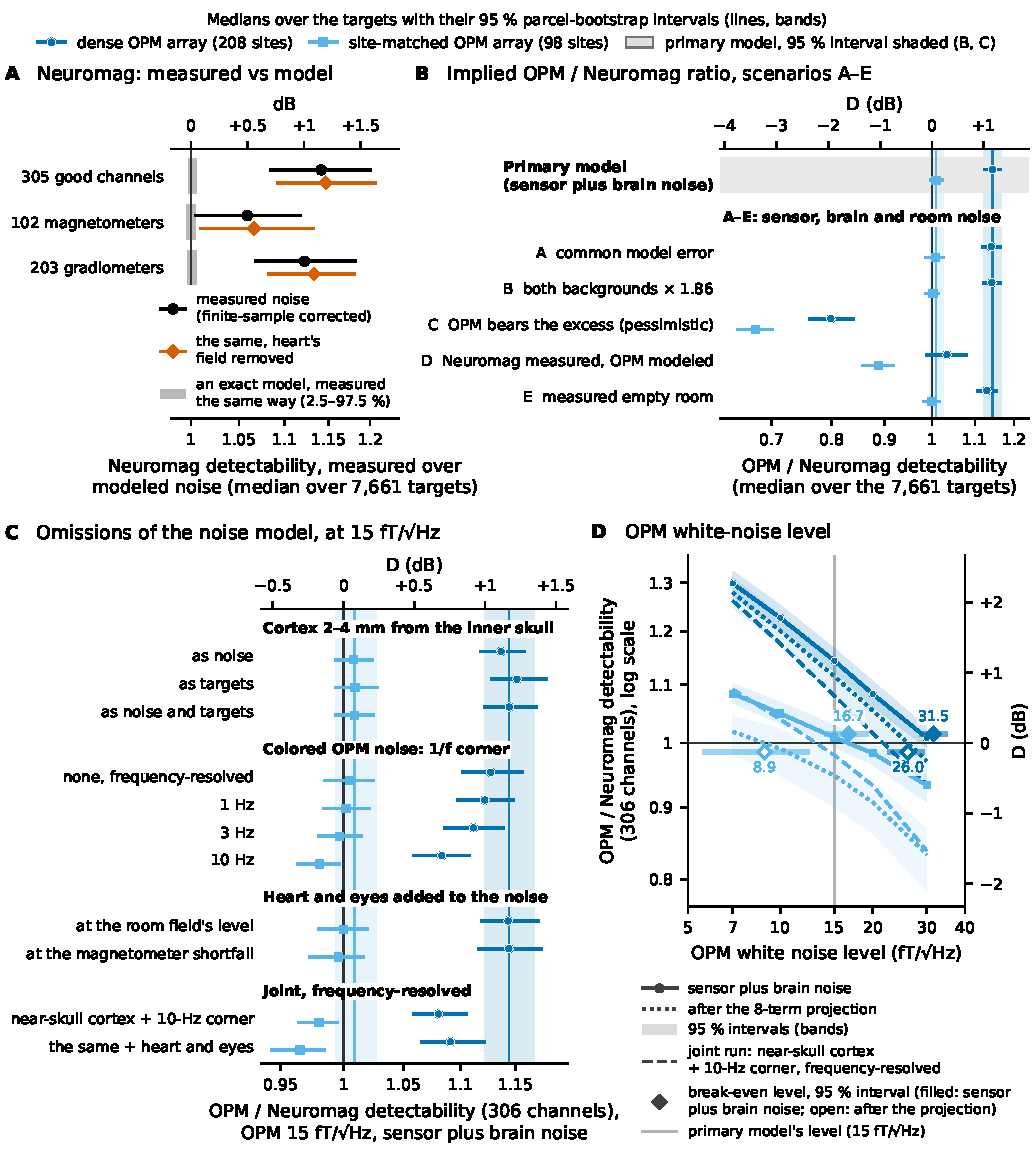
\includegraphics[width=\textwidth,height=0.66\textheight,keepaspectratio]{Figure_3.pdf}
\caption{Determinants of the adult comparison. Median over the 7,661 targets of the target-wise detectability ratio OPM/Neuromag (306 channels) for the dense OPM array (circles), the site-matched OPM array (squares) and a triaxial array at the site-matched sites (triangles, 294 channels), with 95\,\% parcel-bootstrap intervals over 70 atlas labels; logarithmic axis, with $D$ (dB) on the top axis. The gray row and the bands shaded in each array's color mark the primary condition: oracle covariance, sensor plus brain noise, OPM noise of 15~fT/√Hz, no gap beyond the nominal OPM standoff, three-layer BEM and the adult at its measured head position. Each other row changes one factor, except the joint row (30~fT/√Hz with a 3-mm gap). Comparator: Neuromag's 306 channels, gradiometers or magnetometers. Metric: peak-channel SNR; mean-power SNR as an amplitude ratio; and plug-in covariances from 780 or 4,680 independent samples (2BT, twice the bandwidth $B$ times the duration $T$, for $T$ = 10 and 60~s). The single-compartment BEM row uses a subset of targets and has no interval. The columns on the right give the medians.}
\label{fig:conditions}
\end{figure}

\subsection{The noise model against measured Neuromag noise}\label{sec:res-noise}

The model predicted 0.73 of the magnetometers' measured brain-noise amplitude, an independent prediction (Fig.~S2), or 0.89 with the heart's field removed. The gradiometer level at randomly held-out sites (1.00; [0.93, 1.09] over 1,000 splits) and the overall pattern of channel correlations agreed with the measurement, the former nearly by construction. The modeled brain noise was, however, too flat from inferior to superior sites (1.34 and 0.75 when fitted on the inferior or the superior half), and its magnetometer correlations and per-channel variances were poorly predicted.

The measured covariance thus differs from the modeled one in structure as well as in level: the magnetometers' excess over the model lay in a few far-field components (Section~S3). With its measured covariance, Neuromag's detectability was 1.14 [1.08, 1.20] times its modeled value (Fig.~\ref{fig:noise}A), a factor as large as the dense array's whole advantage. What this implies for the OPM depends on its real noise, which no measurement here constrains (Fig.~\ref{fig:noise}B).

If the model's error was common to both systems (scenario A), the ratios remained 1.14 and 1.01. They remained close to these values when both cortical backgrounds were scaled by the magnetometers' variance excess over the model, a factor of 1.86 (scenario B), or when Neuromag's measured empty-room noise was combined with the modeled brain noise (scenario E). With Neuromag taken as measured and the OPM as modeled (scenario D), the dense ratio was 1.03 [0.99, 1.08] and the site-matched ratio 0.89. With the OPM bearing the whole magnetometer variance excess as cortical noise (scenario C, the most pessimistic), the ratios were 0.80 and 0.68.

The omissions we could test moved the advantage little at 15~fT/√Hz (Fig.~\ref{fig:noise}C; Table~S4). The cortex 2--4~mm from the inner skull gave 1.14 when added as background and 1.15 when added as targets. A 1/$f$ component with a 10-Hz corner gave 1.07 under the primary detector and 1.08 under one that also whitens across frequency, and cardiac and ocular sources changed the dense ratio by −1.6\,\% to +1.6\,\%. With near-skull background and the 10-Hz corner together and frequency whitening (the joint run; Fig.~\ref{fig:noise}D, dashed), the ratio was 1.08 [1.06, 1.11] at 15~fT/√Hz, about 1 at 20~fT/√Hz (1.016 [0.997, 1.035]) and 0.93 at 30~fT/√Hz. The primary model gave 1.08 [1.06, 1.11] at 20~fT/√Hz.

\begin{figure}[tbp]
\centering
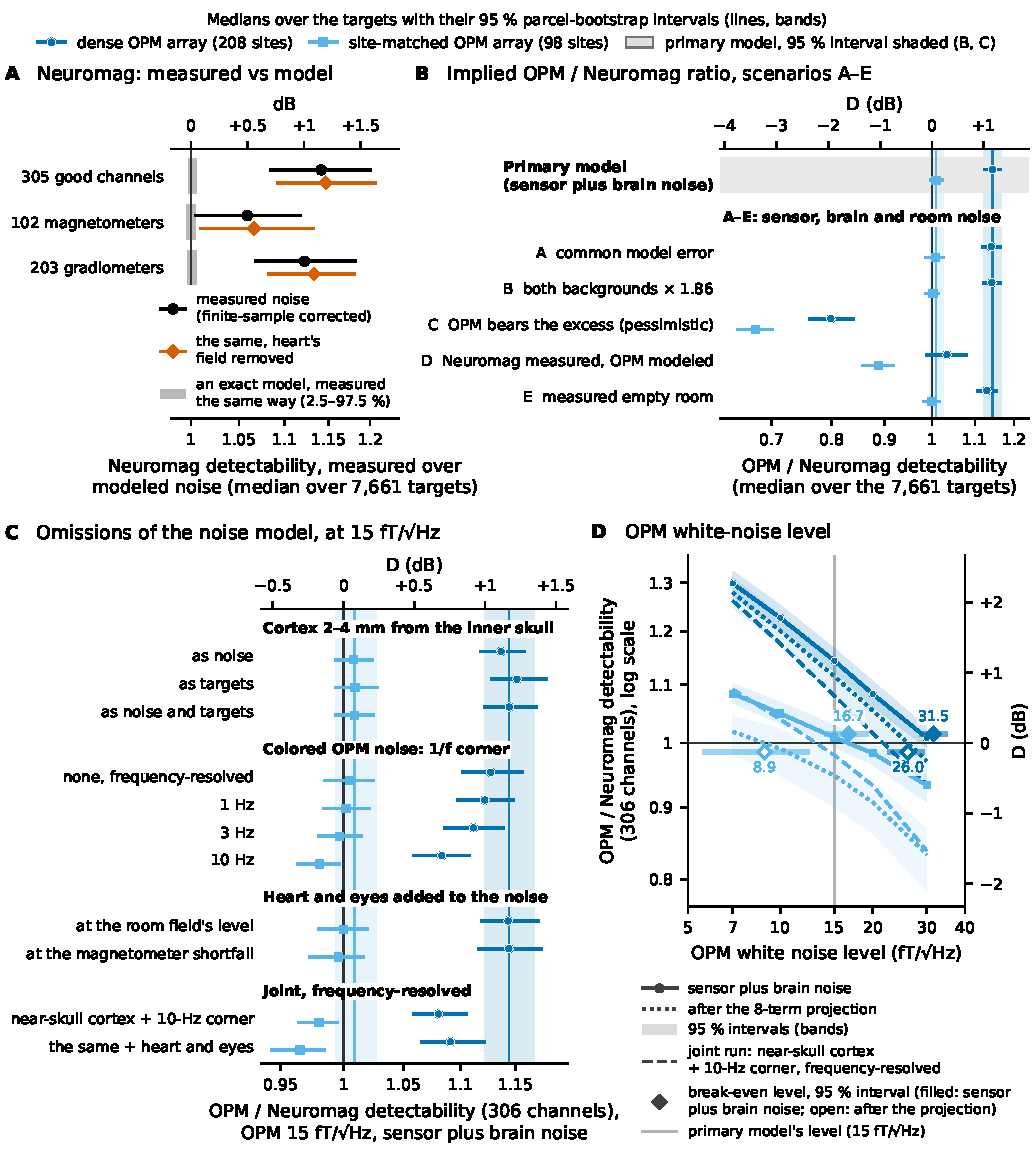
\includegraphics[width=\textwidth,height=0.66\textheight,keepaspectratio]{Figure_4.pdf}
\caption{The noise model against measured Neuromag noise. Adult at its measured head position; medians over the 7,661 targets with 95\,\% parcel-bootstrap intervals (lines, and bands in each array's color); dense OPM array, circles; site-matched OPM array, squares. Ratio axes are logarithmic, with dB on the top or right-hand axis. (A) Neuromag's detectability with its measured noise covariance over that with the modeled one (sensor, brain and room noise; finite-sample corrected) for its 305 channels (one bad channel excluded), the magnetometers and the gradiometers (black), the same with the heart's field removed (orange), and the range an exact model would give when measured in the same way (gray). (B) The implied OPM/Neuromag ratio under scenarios A--E of Section~\ref{sec:res-noise}; gray row, the primary model. (C) The ratio at 15~fT/√Hz when what the model leaves out is added: cortex 2--4~mm from the inner skull as noise, targets or both; colored OPM noise (1/$f$ corners at 1, 3 and 10~Hz); cardiac and ocular sources; and the joint runs. (D) The ratio against the OPM white-noise level with sensor plus brain noise (solid), the room field projected out (dotted) and the joint run of C (dashed), with the break-even levels (diamonds with intervals; filled, sensor plus brain noise; open, projected) and the primary level (vertical line).}
\label{fig:noise}
\end{figure}

\subsection{Depth and brain regions}\label{sec:res-depth}

The dense advantage was largest near the scalp (Fig.~\ref{fig:depth}A): the ratio was 1.60 [1.55, 1.65] in the 10–15~mm bin, 1.13 [1.12, 1.14] at 25–30~mm and 1.05–1.07 from the 35–40 to the 55–60~mm bin, every interval above 1. The site-matched array had an equal-SNR depth even with sensor plus brain noise: its intervals lay above 1 down to the 25–30~mm bin and below 1 from 40–45~mm. With the room field projected out, the dense array's bin median fell below 1 from 45–50~mm and the site-matched array's from 25–30~mm, with intervals below 1 only at 55–60~mm and from 30–35~mm, respectively.

For the dense array, the fall with depth was geometric. It was present with sensor noise alone (Fig.~\ref{fig:depth}A, dotted) and in the peak field itself (Fig.~\ref{fig:depth}B), and brain noise multiplied the ratio by a nearly constant factor in every bin (1.51–1.68). For sources 10–15~mm deep, the dense ratio stayed above 1 under every noise alternative examined. It was 1.35 under scenario D (point estimate), 1.32 [1.27, 1.36] at 30~fT/√Hz, and 1.15 [1.11, 1.21] at 30~fT/√Hz with near-skull cortex, a 10-Hz corner and cardiac and ocular sources added. On the cortex (Fig.~\ref{fig:maps}), the dense array was ahead almost everywhere, most of all on the lateral convexity.

By region (Fig.~\ref{fig:regions}), the dense advantage was largest in the frontal lobe (1.22 [1.18, 1.26]) and smallest in the cingulate (1.05 [1.04, 1.07]) and the insula (1.09). Of the regions chosen from the epilepsy literature, the precentral gyrus favored the dense array most (1.21) and the parahippocampal cortex least (1.12), although 12 atlas parcels, mostly cingulate and medial, had smaller advantages. The site-matched array trailed most on ventral and polar surfaces, such as the frontal pole (0.71), the medial and lateral orbitofrontal cortex (0.78 and 0.79) and the temporal pole (0.83), and, among the literature's regions, in the mesial temporal cortex (parahippocampal and entorhinal; 0.92).

These rankings are exploratory point estimates under the modeled noise. Under scenario D, the dense ratio became 0.75 in the cingulate, 0.96 in the parietal, 1.01 in the frontal and 1.32 in the temporal lobe (point estimates), and its bin medians fell below 1 from the 25–30~mm bin.

\begin{figure}[tbp]
\centering
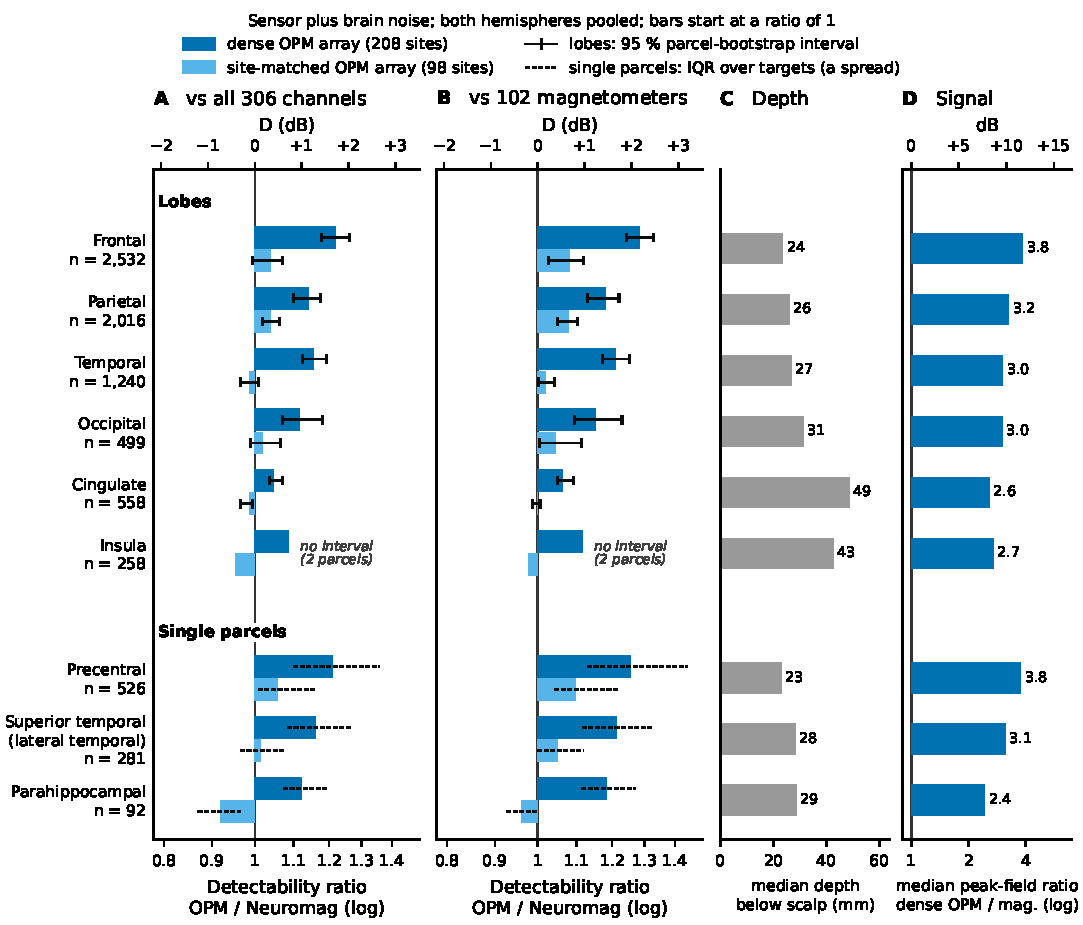
\includegraphics[width=\textwidth,height=0.62\textheight,keepaspectratio]{Figure_5.pdf}
\caption{The adult comparison by depth. (A) Median target-wise detectability ratio OPM/Neuromag (306 channels) in 5-mm depth bins for the dense (208 sites) and site-matched (98 sites) OPM arrays, with sensor noise only (dotted), sensor plus brain noise (solid; the primary condition, its interquartile range, IQR, over targets shaded) and the room field projected out (dashed). Bars: 95\,\% intervals of the bin median from 1,000 resamples of the parcel labels in the bin. Gray numbers: targets per bin (the few targets deeper than the last bin are not drawn). (B) Signal only: peak field of the OPM array over that of the best Neuromag magnetometer (median, IQR and 95\,\% interval per bin), with the analytical sphere at the real median standoffs (dashed) and at the standoffs of the spherical analysis \citep{jas2026} (dotted). Ratio axes are logarithmic, with dB on the right.}
\label{fig:depth}
\end{figure}

\begin{figure}[tbp]
\centering
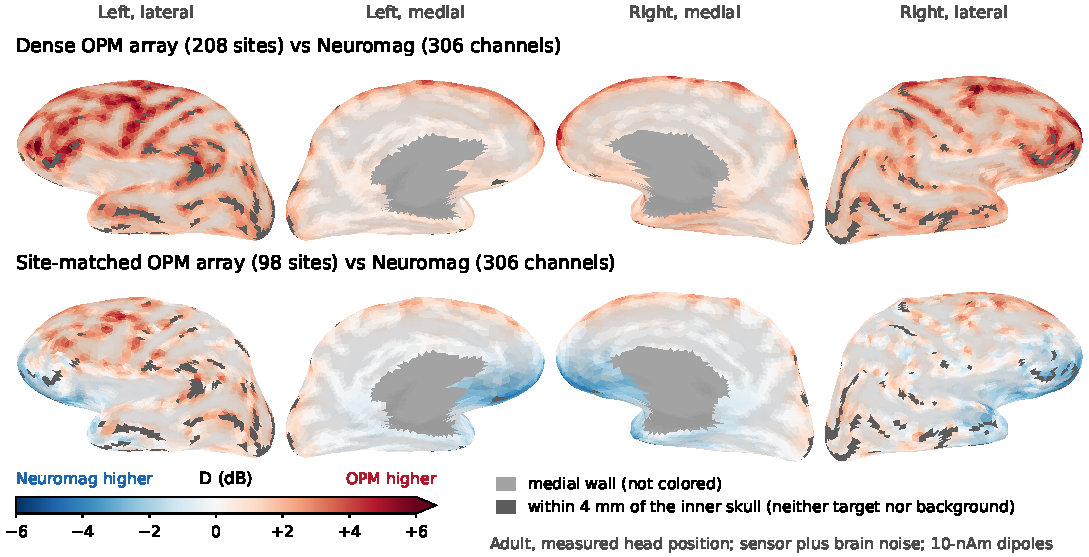
\includegraphics[width=\textwidth]{Figure_6.pdf}
\caption{The adult comparison on the cortex. $D$ on the adult's inflated cortex at its measured head position, sensor plus brain noise, for the dense (top) and site-matched (bottom) arrays against Neuromag's 306 channels; red, the OPM's detectability is higher. Median $D$ is +1.17~dB (dense) and +0.08~dB (site-matched) over all 7,661 targets. Light gray, medial wall (its 558 targets enter the medians but are not colored); dark gray, cortex within 4~mm of the inner skull, neither a target nor part of the background.}
\label{fig:maps}
\end{figure}

\begin{figure}[tbp]
\centering
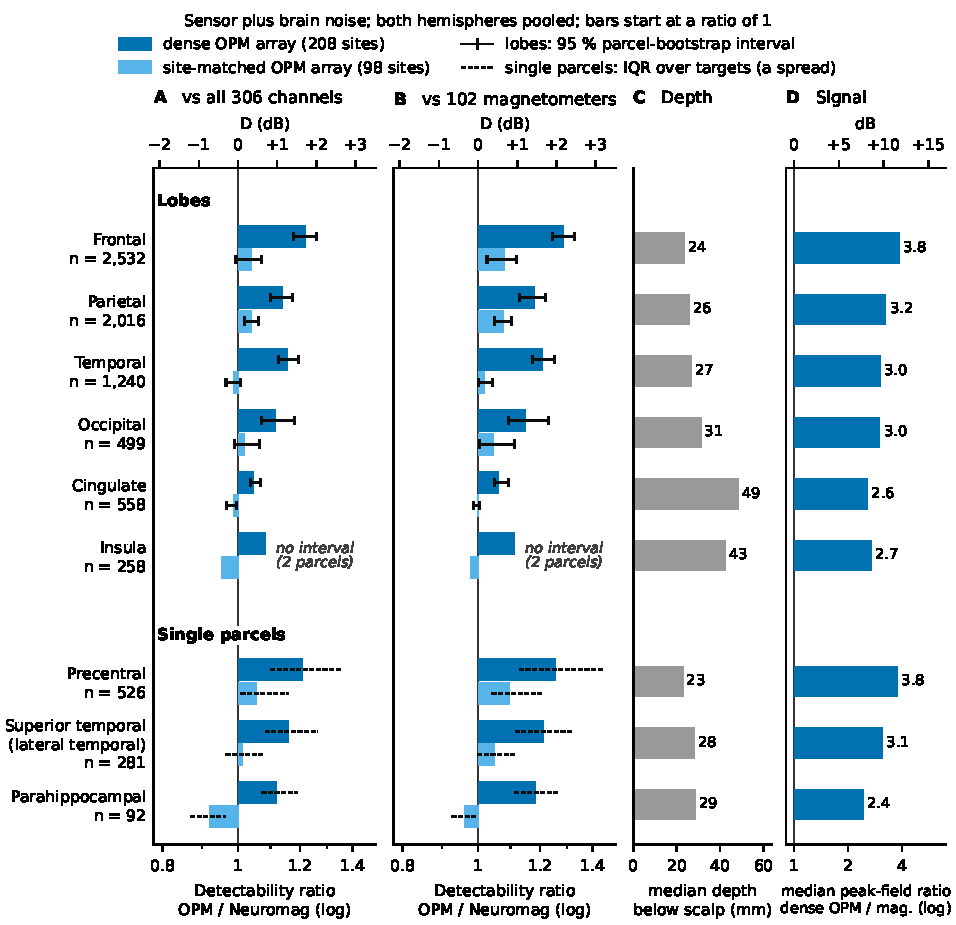
\includegraphics[width=\textwidth,height=0.66\textheight,keepaspectratio]{Figure_7.pdf}
\caption{The adult comparison by brain region. Adult at its measured head position; sensor plus brain noise, OPM noise of 15~fT/√Hz; hemispheres pooled. (A) Median detectability ratio OPM/Neuromag (306 channels) for the dense and site-matched arrays; bars start at 1 on a logarithmic axis, with $D$ (dB) on the top axis. Lobes: median with 95\,\% parcel-bootstrap intervals (solid; the insula, with two parcels, has none). Single parcels (precentral; superior temporal, labeled lateral temporal; parahippocampal): median with the interquartile range over the parcel's targets (dashed), a spread rather than a confidence interval. (B) The same against the 102 magnetometers alone. (C) Median depth below the scalp. (D) Median peak-field ratio of the dense array over the best magnetometer (signal only). Targets per region: 2,532 frontal, 2,016 parietal, 1,240 temporal, 499 occipital, 558 cingulate, 258 insula, 526 precentral, 281 superior temporal and 92 parahippocampal.}
\label{fig:regions}
\end{figure}

\subsection{Smaller heads in the fixed adult helmet}\label{sec:res-heads}

The dense array's $D$ was +1.19 to +2.13~dB in the smaller heads and +1.00 [+0.82, +1.17]~dB in the adult at top contact (Fig.~\ref{fig:heads}A, C). At top contact, the median magnetometer-to-scalp gap was 32.6–40.4~mm in the smaller heads and 28.4~mm in the adult (Fig.~\ref{fig:fit}A; Table~S5). In the scaled adults and infant templates, $\Delta$ was +0.44 to +1.07~dB (Fig.~\ref{fig:heads}B). Placement, which the parcel intervals exclude, mattered as much: over the source-blind placements of the fixed helmet, $\Delta$ spanned +0.20 to +1.12~dB in the school-age scaled adult, and it was positive at every placement in every scaled adult and template (Fig.~\ref{fig:fit}B).

In the school-aged children, provisional examples, $\Delta$ was smaller: +0.30 [+0.11, +0.38], +0.41 [+0.28, +0.54] and +0.17 [−0.07, +0.34]~dB in A, B and C. Over the placements it spanned +0.06 to +0.37, +0.19 to +0.63 and −0.10 to +0.70~dB, and the crossed bands, which set any placement of the child against any of the adult's, included zero in every child (Section~S5).

\begin{figure}[tbp]
\centering
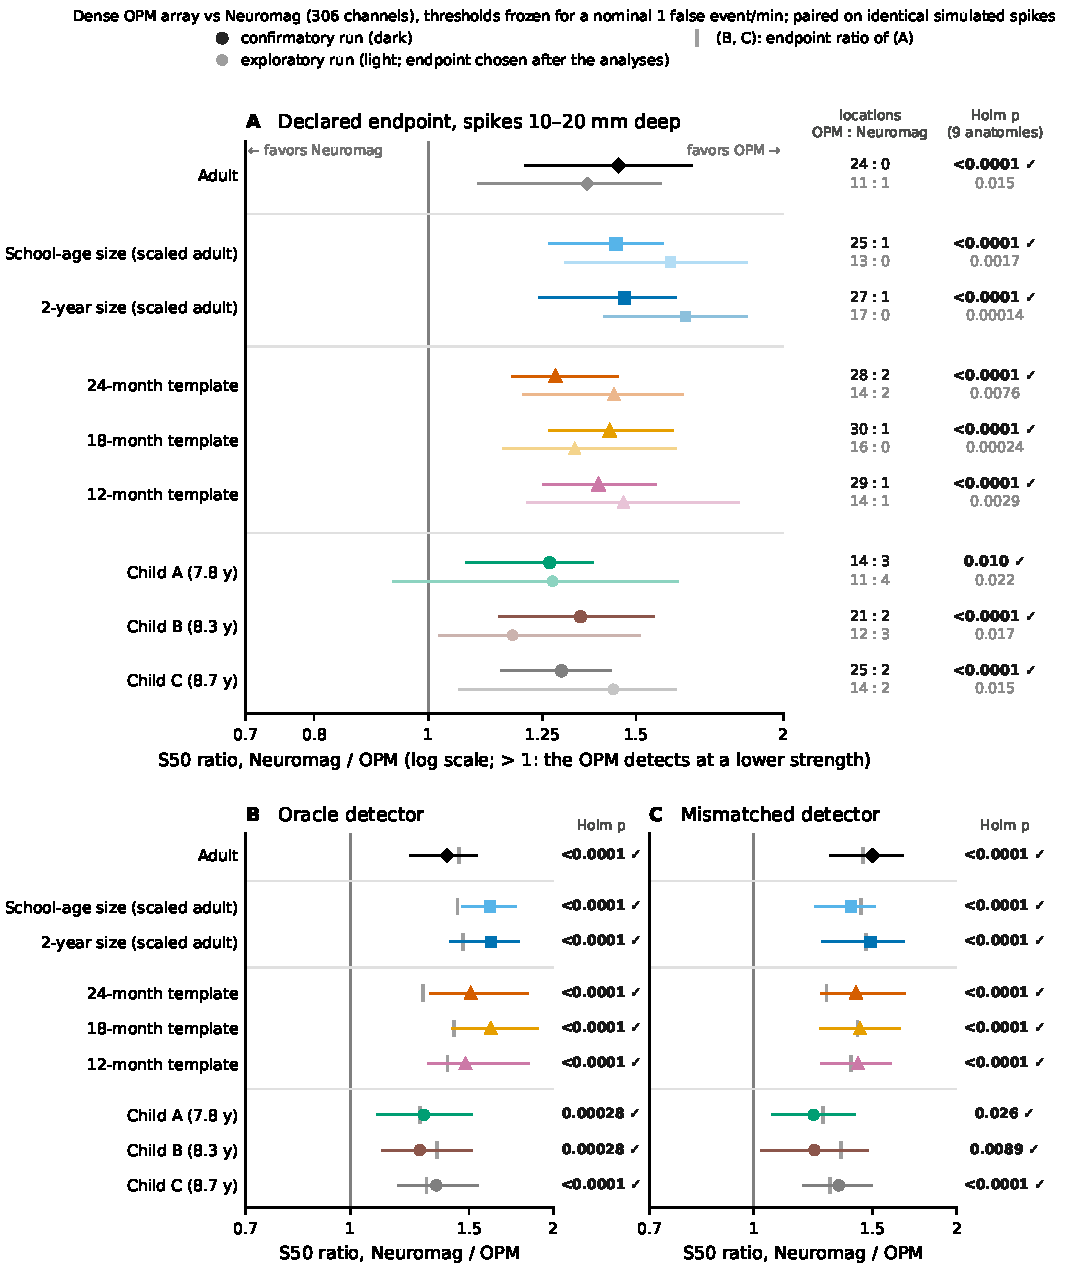
\includegraphics[width=\textwidth,height=0.6\textheight,keepaspectratio]{Figure_8.pdf}
\caption{Smaller heads in the fixed adult helmet. Dense OPM array against Neuromag (306 channels) at top contact; $D$ is the area-weighted median over cortical targets, medial wall excluded. (A) $D$ for the eight smaller heads with sensor plus brain noise (filled) and with the room field projected out (open), with 95\,\% parcel-bootstrap intervals; vertical lines, the adult's $D$ at top contact (+1.00 and +0.86~dB). (B) $\Delta$ with 95\,\% parcel-bootstrap intervals (1,000 resamples). Heads are grouped by class and ordered by head circumference (the number after each label); squares, scaled adults; triangles, infant templates; circles, school-aged children (provisional examples); one color per head, as in Fig.~\ref{fig:confirm}. (C) $D$ on the inflated cortex of the 24-month and 12-month infant templates (dense arrays of 151 and 144 sites), on the color scale of Fig.~\ref{fig:maps}; values beyond ±6~dB take the end color (3.3\,\% and 6.1\,\% of the cortical targets lie above +6~dB). The 18-month template is classed misregistered by the MRI check. Infant templates: \citet{oreilly2021}, from the Neurodevelopmental MRI Database \citep{richards2016}; children A--C: OpenNeuro ds005234 \citep{fadeev2024,fadeev2025}.}
\label{fig:heads}
\end{figure}

\subsection{Helmet fit versus head size}\label{sec:res-fit}

The interaction measures how much more the fixed helmet favors a smaller head than the adult, relative to the helmet fitted at the adult's gap. It was +0.40 to +1.10~dB in the scaled adults and templates, every interval above zero (Fig.~\ref{fig:fit}C; per head in Table~S6). The two scaled adults gave the lowest and the highest values (+0.40 and +1.10~dB) and the templates +0.54 to +0.70~dB. The interaction exceeds the heads' own within-head contrasts (+0.17 to +0.76~dB) because the adult's contrast is negative, −0.23~dB: the fitted helmet holds the adult laterally centered, a looser pose than top contact.

In the fitted helmet, little of the excess remained (Fig.~\ref{fig:fit}B). Against the adult fitted the same way, $\Delta$ was +0.02 to +0.15~dB in the scaled adults and templates (point estimates; interval bounds −0.09 to +0.33~dB). Every template interval included zero, only the school-age scaled adult's lay just above it, and the highest value was that of the 18-month template. Fitted instead at the adult's top-contact gap, these heads kept +0.10 to +0.23~dB against the adult at top contact (Section~S5). With the room field projected out, every smaller head's point estimate at the adult's gap lay below the adult's (−0.67 to −0.05~dB; three of the eight intervals including zero).

None of these quantities apportions the effects exactly, because the fitted helmet changes the gap distribution, the placement and the sensors' coverage together. In the fitted helmet and at equal OPM site count, $\Delta$ was +0.16 to +0.49~dB (Section~S5); in the scaled adults and templates, their fewer OPM sites offset a similar amount. In the children, $\Delta$ at the adult's gap was negative in A and B (−0.30 [−0.48, −0.22] and −0.39 [−0.54, −0.17]~dB), but not against the adult at top contact (−0.11 [−0.40, +0.06] and −0.22 [−0.35, +0.01]~dB). In child C, whose two gaps nearly coincide, it was +0.01 [−0.23, +0.18]~dB.

\begin{figure}[tbp]
\centering
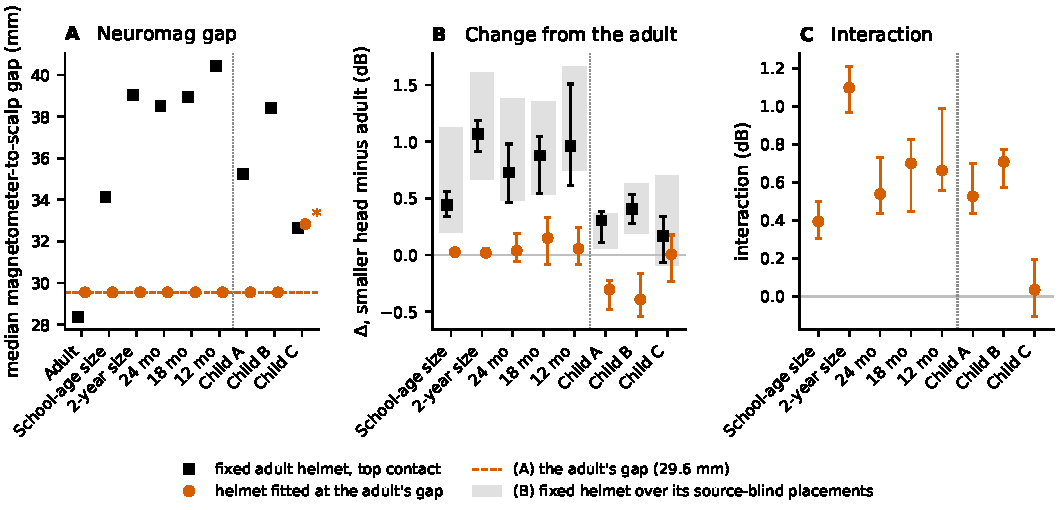
\includegraphics[width=\textwidth]{Figure_9.pdf}
\caption{Helmet fit versus head size. Dense OPM array against Neuromag (306 channels), sensor plus brain noise; bars, 95\,\% intervals from parcels resampled within each head. Filled black squares, the fixed adult helmet at top contact; filled vermillion circles, the helmet fitted at the adult's gap (Section~\ref{sec:arrays}; asterisk, child C, where the 18-mm limit binds). (A) Median magnetometer-to-scalp gap in each helmet; dashed line, the adult's gap when laterally centered (29.6~mm). (B) $\Delta$ against the adult placed by the same rule in each helmet; gray ranges, $\Delta$ at each feasible one of the 12 source-blind placements of the fixed helmet (11 in child C), as a difference of medians. (C) The interaction, the primary helmet-fit quantity: a head's within-head contrast between the two helmets minus the adult's, taken per vertex or parcel; it does not depend on the OPM noise. The dotted line sets apart the school-aged children, provisional examples. Head labels: School-age size and 2-year size, the scaled adults; 24, 18 and 12~mo, the infant templates; the 18-month template is classed misregistered by the MRI check.}
\label{fig:fit}
\end{figure}

\subsection{Simulated interictal spikes}\label{sec:res-spikes}

In the pre-specified run, the S50 ratio Neuromag/OPM was 1.27–1.47 across the anatomies, every location-bootstrap interval above 1 (Fig.~\ref{fig:confirm}A; Table~S11): under the modeled noise, the dense array detected spikes 10–20~mm deep at 21–32\,\% lower strength. The declared sign-flip test favored the dense array in every anatomy (Holm-adjusted p at most 0.0103). In the adult, the S50 ratio (1.45) was of the order of the detectability ratio at these depths (1.36--1.60; Fig.~\ref{fig:depth}A). The ratios varied little across the five noise replicates (standard deviation 2.9–6.4\,\%; pooled ratios 1.22–1.44).

The result did not hinge on the practical detector's thresholds. The oracle detector, whose realized per-trial false-positive probability on held-out null data was 0.00093–0.0011, gave ratios of 1.27–1.62 (Fig.~\ref{fig:confirm}B). At the frozen thresholds, separate null data that no threshold had seen gave 0.90–2.15 false events per minute for the dense array and 0.70–2.25 for Neuromag. An approximate equal-rate test (uncorrected; the arrays share their background and room noise) gave p < 0.05 in two anatomies (Section~S7). With each threshold re-fitted on held-out null data to the nominal 1 false event per minute (realized rates 0.90–1.60 and 0.70–1.45), the ratios were 1.27–1.50.

The mismatched detector changed the ratio by a factor of 0.91–1.11, every interval including 1 (Fig.~\ref{fig:confirm}C); with rate-matched thresholds, its test favored the dense array in 8 of 9 anatomies (child B, Holm-adjusted p = 0.072). The site-matched array's S50 ratios were 0.99–1.30, above 1 by point estimate in 8 of 9 anatomies, in line with its shallow advantage (Section~\ref{sec:res-depth}). The exploratory run gave concordant results (S50 ratios 1.18–1.65 over 18 locations per anatomy in this band); its deeper bands are reported in Section~S7. Spike detection was not simulated under the noise alternatives of Section~\ref{sec:res-noise} or in the fitted helmet.

No localization difference was established in the exploratory run. Dipole fits of detected 320-nAm focal spikes had median errors of 3.7–7.6~mm in every array and anatomy, of the order of the coregistration displacement (2.1–3.2~mm). Of 360 paired comparisons of dipole and dSPM errors and of joint detection and localization, 65 reached p < 0.05 uncorrected (about 18 expected by chance; 61 favoring an OPM array). Of these, 8 survived a Bonferroni correction within anatomy and array, and 0 survived one over all 360 (Section~S7; Fig.~S14).

\begin{figure}[tbp]
\centering
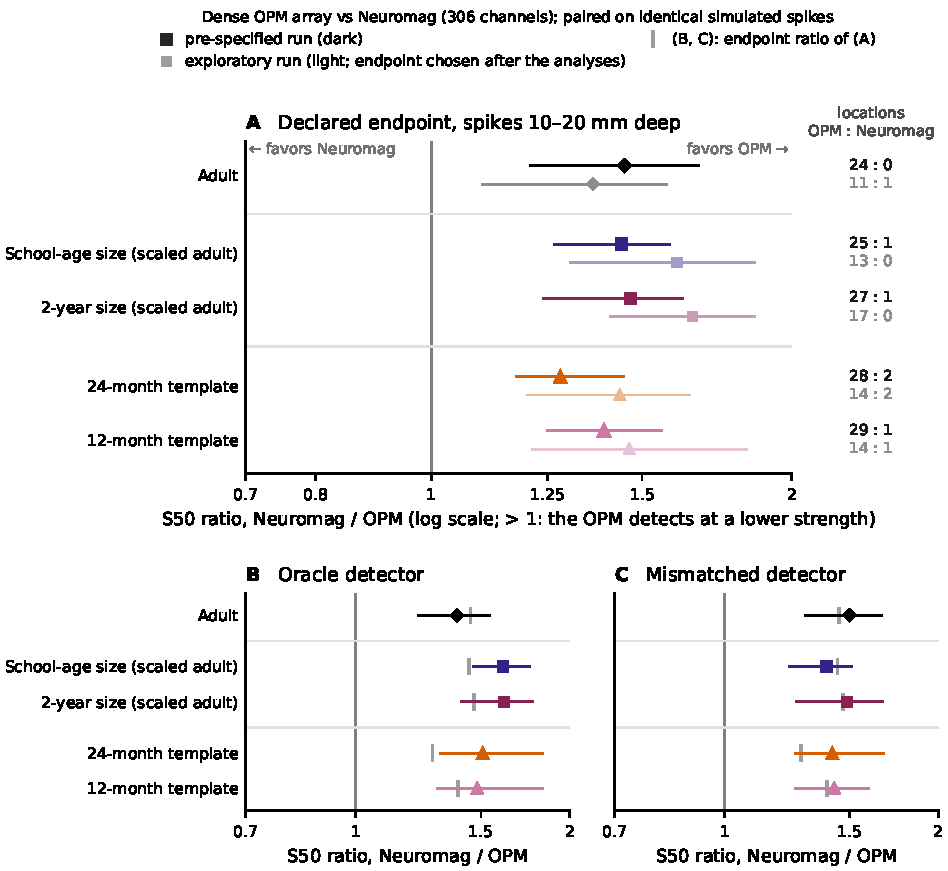
\includegraphics[width=\textwidth,height=0.62\textheight,keepaspectratio]{Figure_10.pdf}
\caption{Simulated interictal spikes: the pre-specified run. S50 ratio (S50, the dipole strength detected in 50\,\% of events), Neuromag (306 channels) over the dense OPM array, for focal spikes 10–20~mm below the scalp at 36 newly drawn locations per anatomy (648 focal events; the first of five noise replicates); logarithmic axis (above 1, the OPM detects at a lower strength); lines, 95\,\% location-bootstrap intervals (1,000 resamples). (A) The declared endpoint: the practical scanning detector, idealized in that it uses the true forward model and the simulated waveform family, with thresholds frozen for a nominal 1 false event per minute (dark markers). Right: the numbers of locations at which the OPM or Neuromag detected more events (the others are ties) and the two-sided sign-flip p, exact and Holm-adjusted over the anatomies. Light markers: the exploratory run (18 locations per anatomy; endpoint chosen after the analyses). (B) The oracle detector (known source, waveform and time; per-trial false-positive probability 0.001). (C) The mismatched detector (Section~\ref{sec:spikes}). In B and C, gray bars mark the endpoint's ratio of A. Diamond, the adult at its measured head position; other heads at top contact in the fixed adult helmet, with symbols and colors as in Fig.~\ref{fig:heads}; the children's rows are provisional examples.}
\label{fig:confirm}
\end{figure}

\FloatBarrier
%% =====================================================================
\section{Discussion}\label{sec:discussion}

Three findings are the firmest of this study. First, which system leads is decided by the array design, the OPM noise floor, the Neuromag channels used as comparator and the SNR measure, not by the OPMs' proximity alone. Second, the break-even OPM white noise, 31.5~fT/√Hz for a dense array and 16.7~fT/√Hz at Neuromag's sites, is a prediction that measured OPM noise can test. Third, most of the extra advantage of smaller heads in the adult helmet disappears when the helmet is fitted to the adult's gap, a contrast that depends on the SQUID helmet alone. The dense array's adult advantage itself is no larger than the model's error for Neuromag, and under the model it carries over to the detection of superficial spikes.

\subsection{What decides the adult comparison}\label{sec:disc-noise}

The spherical analysis of \citet{jas2026} places the OPM advantage within an equal-SNR depth set by an assumed noise ratio. With explicit noise, the dense array has an advantage at every depth. It shows an equal-SNR depth only after the room projection (by bin medians, with an interval below 1 only at 55–60~mm) or with Neuromag's measured noise (scenario D, point estimates), whereas the site-matched array keeps one even with sensor plus brain noise. Depth therefore changes the size of the dense advantage and the sign of the site-matched array's, while the OPM noise floor and the array can reverse which system leads.

Brain noise turns the SQUID advantage into an OPM advantage. Its size is consistent with the per-channel noise budget: brain noise raises the noise of a Neuromag magnetometer about 9.3-fold over its low sensor floor but that of an OPM only about 5.7-fold (Section~S3). The OPM's higher sensor noise therefore matters less once brain noise dominates. The comparator and the metric then decide how a reported number shows the difference: a peak-channel SNR against magnetometers favors the OPM, one against the best of all channels favors Neuromag, and a channel-averaged SNR shows little difference.

The size of the dense advantage cannot be fixed more tightly than the model's error for Neuromag. Depending on how the OPM shares that error, the five scenarios placed the dense ratio between 0.80 and 1.14. Because OPMs are magnetometers, their real noise may share some of the far-field excess that the model misses for Neuromag's magnetometers. The truth then lies between an error common to both systems (scenario A) and the OPM bearing the whole excess (scenario C), and scenario D, with a dense ratio of 1.03 [0.99, 1.08], is a plausible central case rather than a pessimistic extreme. The break-even noise levels are the study's testable predictions: a measured OPM noise covariance in the same band would place a real array above or below them directly.

The regional pattern is exploratory and rests on the modeled noise. Under that noise, the dense advantage is largest on the frontal and central convexity and smallest in cingulate cortex, and the site-matched array trails on ventral and polar surfaces, including the mesial temporal cortex. Under scenario D, the frontal advantage falls to about 1, the cingulate and parietal lobes fall below 1, and the temporal lobe leads.

\subsection{Head size and helmet fit}\label{sec:disc-fit}

The spherical analysis predicts a larger OPM benefit in smaller heads, because a shell at a constant standoff leaves more of a small brain within the equal-SNR depth \citep{jas2026}. In the fixed adult helmet, the scaled adults and templates did gain more than the adult. Fitting the helmet to each head at the adult's gap removed most of this excess (an interaction of +0.40 to +1.10~dB). Because the interaction compares two Neuromag helmets around the same OPM array, this result, unlike the others of this study, does not depend on the unmeasured OPM noise. In this model, the sphere's prediction thus holds in the adult helmet but largely reflects how that helmet fits a smaller head, its gap, placement and coverage together; the construction does not isolate the median gap, or exclude head size, as a cause.

The scaled adults carry this conclusion, because they keep the adult's anatomy: their fixed-helmet excess of +0.44 and +1.07~dB fell to +0.13 and +0.11~dB against the adult at top contact when the helmet was fitted at the adult's top-contact gap. What remains in the fitted helmet depends on the adult's reference placement and, for the templates, on their scalp convention (Section~\ref{sec:limitations}). At equal OPM site count, $\Delta$ was +0.16 to +0.49~dB, the quantity comparable to the sensor-noise-only result of \citet{zahran2022}, and the smaller heads' fewer OPM sites offset a similar amount.

For pediatric MEG, these results suggest that much of the extra on-scalp advantage that small heads show in an adult helmet reflects that helmet's fit. Our fitted helmet keeps the adult's sensors and does not model a pediatric SQUID system, such as one built for young children \citep{tesan2010}, and how a child is positioned in an adult helmet matters as well \citep{gaetz2008}. The school-aged children did not change this picture, but their anatomy near the scalp could not be verified, and their values remain provisional examples.

\subsection{Simulated spikes and the clinical literature}\label{sec:disc-clinical}

Under the modeled noise and with an idealized detector, the dense array detected superficial spikes at a lower strength than Neuromag in every anatomy. In the adult, the S50 ratio tracked the detectability ratio at those depths, and the ranking survived the declared detector mismatch and a change of thresholds. The spike simulations therefore show that the detectability difference carries over to detection; they do not test the noise model. Under the noise alternatives that were examined for detectability, the dense ratio for sources 10–15~mm deep remained 1.15--1.35 (Section~\ref{sec:res-depth}). The detection advantage for superficial spikes would therefore be expected to shrink under them but not to reverse, an inference from detectability rather than a simulated result. No localization difference was established; dipole-fit errors were of the order of the coregistration error, which may have dominated the comparison.

The clinical reports and the model are compatible, but the model cannot identify which factor operated in any study (Table~S19 sets each study beside its closest model analogue). Higher or similar OPM SNR against SQUID magnetometers (\citealp{feys2022}; mixed results in \citealp{feys2025}) corresponds to the model's peak-channel SNR against the magnetometers, which favors the OPM in every head (Section~S6). Equal or lower SNR against planar gradiometers or the nearest channels of few or noisier sensors \citep{hillebrand2023,schwartz2025} corresponds to peak-channel SNR against the gradiometers or the best channel. The larger gains reported in school-aged children in an adult helmet \citep{feys2022} are compatible with the fixed helmet's fit. The weaker OPM results for temporal and mesial temporal sources \citep{feys2024,feys2025,shen2026} have two analogues in the model, the weakness of deep sources for every system and the site-matched array's deficit on ventral and polar surfaces. The second is fragile, because the model overstates Neuromag's detectability in the temporal lobe (measured over modeled, 0.89; Section~S3).

Clinical arrays reach about 100--128 channels with dual- or triaxial sensors at fewer sites, between the two arrays modeled here. The site-matched array (98 single-axis sites) showed no advantage by whole-cortex detectability at 15~fT/√Hz and a SQUID advantage when noisier, and its small advantages depended on the comparator, the metric, the covariance estimate or depth (within about 30~mm of the scalp). With three axes at the same sites, the ratio rose to 1.12, close to the dense array's, so the model brackets a clinical array without determining where it falls. The modest whole-cortex advantage belongs to an array with more sites than any used in epilepsy so far, at a white noise within the clinical range.

\subsection{Limitations}\label{sec:limitations}

This study has limitations. First, no measurement validates the OPM covariance, and the model's background, calibrated on Neuromag's gradiometers, misses part of the magnetometers' noise; a measured OPM noise covariance, recorded in conditions matched to those of the calibrating recording, would test the predicted advantage and the break-even levels. Second, a single projection stands in for the preprocessing of real systems \citep{taulu2006,tierney2021}, and clinical dual- and triaxial arrays were not modeled; simulating each system's own interference suppression and a clinical array would narrow the bracket. Third, one adult is the reference (its $D$ spans 0.46~dB over the 12 source-blind placements), and the parcel intervals exclude between-subject and placement variability. The pediatric results rest on two copies of the adult, three templates and three children from one dataset; a cohort of individual pediatric MRIs would test them. Fourth, the children's skull is modeled and their fiducials are transferred, and the MRI check can neither verify their white surface within a few millimeters of the scalp nor detect a head boundary that the T1 images themselves place too deep. Fifth, the templates' scalps lie 1.3–1.6~mm outside their MRI head boundaries and the adult's 1.3~mm inside. This difference of conventions, 2.6–3.0~mm, could lower the templates' $D$ and $\Delta$ (for illustration, a 3-mm OPM gap lowers the adult's dense ratio from 1.14 to 1.09), although the interaction, a difference of contrasts on one scalp, is less exposed to it. The 18-month template's surface also fits its T1 image best after a 2.3-mm shift, whose effect on its $\Delta$ was not estimated. Sixth, the smaller heads keep the adult's background variance per unit cortical area; with that variance halved or doubled, every smaller head's median $D$ still exceeded the adult's in the fixed helmet (by +0.25 to +1.18 and +0.11 to +1.07~dB). Seventh, all sources lie on the cortical surface, so the hippocampus and amygdala are absent. Finally, the spike simulations use the simulation's own stationary model for the detector's templates, candidate patterns and whitening, and the null data hold no physiological transients. The threshold-calibration uncertainty is not propagated into the S50 intervals, and spikes were simulated neither under the noise alternatives nor in the fitted helmet; recordings of real or phantom spikes with both systems would test the detection result.

\FloatBarrier
%% =====================================================================
\section{Conclusions}\label{sec:conclusions}

With explicit noise in a realistic adult head, the advantage of on-scalp OPMs over the Neuromag system depended on array design, OPM noise, comparator and metric. A dense array of 15-fT/√Hz OPMs had a modestly higher detectability up to a break-even noise of 31.5~fT/√Hz, and an array at Neuromag's sites showed no advantage. The dense advantage is as large as the model's error for Neuromag, so measured OPM noise must decide it. In smaller heads, fitting the helmet to the adult's gap removed most of the extra advantage that the scaled adults and templates showed in the fixed adult helmet, a result that does not depend on the OPM noise. Under the modeled noise and with an idealized detector, the dense array detected weaker superficial simulated spikes in every anatomy. Clinical reports of higher OPM SNR are compatible with these conditions, which the model cannot tell apart in any single study.

%% =====================================================================
\section*{CRediT authorship contribution statement}

\textbf{Laiba Khan:} Conceptualization, Methodology, Software, Formal analysis, Investigation, Data curation, Visualization, Writing -- original draft. \textbf{Mainak Jas:} Conceptualization, Supervision, Writing -- review \& editing.

\section*{Declaration of competing interest}

The authors declare that they have no known competing financial interests or personal relationships that could have appeared to influence the work reported in this paper.

\section*{Funding}

This research did not receive any specific grant from funding agencies in the public, commercial, or not-for-profit sectors.

\section*{Data and code availability}

The analysis code, configurations and tests are available at \url{https://github.com/khan-laiba/opm-squid-meg} under the MIT license, and the result files (JSON and CSV, in the repository's results folder) and figures under the CC BY 4.0 license. The external data are not redistributed but are obtained from their sources with the repository's fetch scripts: the MNE sample dataset \citep{gramfort2013}, in the processed release that the dataset fetcher of MNE-Python 1.13.2 downloads (OSF file 86qa2, version 6); the infant templates \citep{oreilly2021,richards2016}, through MNE-Python's template fetcher (LGPL-2.1); and the MRIs and surfaces of the children, OpenNeuro ds005234, version 2.2.0 \citep{fadeev2025}, whose metadata give CC0 and whose authors ask that it be acknowledged as distributed under CC BY with its DOI. The documentation of the sample dataset restricts it to learning the software and advises against using it to evaluate the MEG or MRI system. Here, the recording calibrates the noise model and its measured covariance serves as a check of that model, and the values are not offered as an evaluation of the VectorView system or of the MRI scanner.

\section*{Ethics statement}

This simulation study used only publicly available, de-identified data collected under the approvals of the original studies; no new data were collected from human participants. Sex and gender were not analyzed: with one adult, three averaged templates and three children, the head models are too few for any analysis by sex.

\section*{Declaration of generative AI and AI-assisted technologies in the manuscript preparation process}

During the preparation of this work the authors used Claude (Anthropic) to write and run the analysis code and to draft and edit the manuscript. After using this tool, the authors reviewed and edited the content as needed and take full responsibility for the content of the publication.

\bibliographystyle{elsarticle-harv}
\bibliography{references}

\appendix
\section{Supplementary material}\label{app:supp}

Supplementary material related to this article is provided as a separate file. It comprises Sections~S1--S9 (estimands and conventions; the spherical benchmark; the noise model's components, calibration, validation and sensitivity analyses; the head models and the MRI check; the helmet constructions; regions and the noise floor across heads; the spike study; the parameters, the analysis choices made after results were known, the literature search and the parameters' provenance; and the clinical OPM studies with their model analogues), Figs.~S1--S15 and Tables~S1--S19.

\end{document}
